\documentclass[12pt,a4paper]{article}
\usepackage[utf8]{inputenc}
\usepackage[portuguese]{babel}
\usepackage[T1]{fontenc}
\usepackage{graphicx}
\usepackage{amsmath}
\usepackage{lipsum}
\usepackage{float}


\begin{document}



\title{{\Huge \textbf{Otimização da Intreção de Gauss}}}
\author{Mateus Akira Moraes Yamaoka}
\maketitle


\newpage
\section{Introdução}
\qquad A integração numérica pode ser feita de vários modos, como já foi estudado na primeira parte desse relatório, e para o prosseguimento do estudo foi escolhida a Integração de Gauss como o método mais eficiênte para essa integração. Contudo, foi visto que a integração de Gauss exige um valor mínimo de pontos de integração para que sua aproximação seja precisa. Nesse sentido, sempre que se for utilizar esse método para a aproximação é necessário saber o número de pontos mínimos necessarios para que se calcule o valor da integral suficientemente próximo ao valor real e também que não sejam utilizados muito mais pontos do que o necessário, fazendo assim que a operação seja computacionamente mais barata.




\newpage
\section{Objetivos}

\qquad O projeto de iniciação científica objetiva a otimização da integração numérica de uma função, ou seja, ajustar a integração de forma a usar o menor número de pontos de integração possível para um intervalo, afim de obter o resultado com a margem de erro consideravelmente baixa. Desse modo, esse estudo foi realizado com o intuito de elaborar uma abordagem amtemática que desempenhasse essa função.


\newpage
\section{Metodologia e Resultados}
\qquad A metodologia para esse estudo foi dividia em algumas partes. Primeiramente, foi pensando em um modelo que serviria de base de comparação de resultados, ou seja, um modelo que , mesmo que com maior esforço computacional, retornasse qual seria o menor número de pontos de integração para uma determianada função e intervalo de integração.

Depois disso, foi então pensando em um modelo que retornasse um valor próximo ao primeiro, mas com menor esforço computacional.
\subsection{Criação de um método comparativo}

\qquad Para a criação do método GaussNumber, que serivirá de base para saber o valor mínimo necessário do número de pontos de integração, foi baseado em se resolver a própria integração de Gauss para alguns valores e comparar o resultados entre eles. Inicia-se a integração com um ponto de integração e compara-se o resultado dassa integração com o valor da integração usando n+1 pontos de integração. Caso a difrença entre eles seja menor que um valor adotado $10^{-10}$, o método para e retorna como o valor mínimo de ingreção o n+1, caso contrário o método continua a comparação, agora entre n+1 e n+2, e assim por diante.

Assim, levando em consideração somente o intervalo de integração e a função, apesar de um grande esforço computacional, foi possível saber qual o valor mínimo a ser usado na integração de Gauss de modo que o resultado seja muito próximo do valor da integração de fato.

\newpage
\subsection{Criação do modelo otimizado}
\qquad Foi percebido que conforme a função tenha um comportamento mais parecido com o de uma função linear, menores são os números de pontos de integração necessários para se aproximar a integração. Esse comportamento chamou a anteção para o estudo das derivadas de algumas ordens das funções, pois conhecendo as derivadas da função é possível saber se em algum momento uma dessas derivadas seria constante ou igual a zero, indicando que a função seria de baixa ordem e poderia ser aproximada por um número de pontos de integração já predertimando.

Assim, o primeiro passo dessa metodologia foi o estudo das derivadas. Para isso foi usado o método numérico para obtenção da derivada, que consiste no cálculo da secante usando um ponto da função e um próximo ponto distante "h" desse primeiro, como mostra a imagem a seguir:


\begin{figure}[h]
\begin{center}
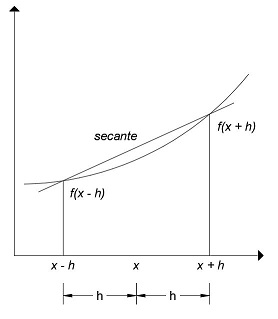
\includegraphics{images/derivative}
\end{center}
\caption{Ilustração do método de derivação numérico.}
\end{figure}



O método usado é mostrado a seguir como exemplo do cálculo da primeira derivada(dfdx1), em que "h" foi um valor adotado como $10^{-4}$:

\begin{equation}
dfdx1=\frac{f(x+h)-f(x-h)}{2\times h}
\end{equation}

Foram considerados os valores absolutos das derivadas, pois a indicação de uma inclinação ascendente ou descendente não é importante para esse estudo,

Seguindo essa ideia, foram também calculados os valores das derivadas até a quinta ordem, seguindo o seguinte modelo exemplificado para a segunda derivada (dfdx2).

\begin{equation}
dfdx2=\frac{dfdx1(x+h)-dfdx1(x-h)}{2\times h}
\end{equation}

Assim, com os valores calculados até a quinta derivada foi possível analisar seus resultados. Pra isso foi primeiramente utilizado o método GaussNumber para se obter o número exato de pontos de integração para equações polinomiais de primeira até terceira ordem (onde a derivada de quinta ordem é igual a zero). Para cada uma das ordens das derivadas, se o valor dessas for menor do que $\beta = 10^{-4}$, foi considerado como sendo zero. Isso implica que para cada uma das derivadas sendo zero, o número de pontos de integração varia, conforme a tabela a seguir:

\begin{center}
    \begin{tabular}{| c | c |}
    \hline
    Caso & Número de pontos necessários\\ \hline
    dfdx1 = 0 & 1 \\ \hline
    dfdx2 = 0 & 1 \\ \hline
    dfdx3 = 0 & 2 \\ \hline
    dfdx4 = 0 & 2 \\ \hline
    dfdx5 = 0 & 3 \\ \hline
    dfdx5 > 0 & MaxAvailable \\ \hline
  
    \hline
    \end{tabular}
\end{center}

Para o caso em que dfdx5>0, o método retornara um valor denominado MaxAvailable, que significa o maior valor adotado para o número de pontos de integração. Entendendo-se que não há necessidade de realizar a operação com um valor maior que 10, pois o resultado com 10 pontos já será satisfatório. 

Esses valores são usados no cálculo do número de pontos de integração da seguinte forma: ao analisarmos os limites de integração, analisa-se as derivadas nesses dois pontos e usa-se como o valor mínimo de pontos de integraçao para o intervalor, o menor valor entre o retorno desses dois pontos, e como máximo o maior valores desses dois retornos. Caso ambos retornem o valor "maxavailable", o valor mínimo de integração é 3, pois temos um caso em que dfdx5 > 0.

Dados os limites superiores e inferiores da análise, foi pensado então no método para determinar o valor no númeor de pontos de integração. Para isso, Para esse método foram levados em considerações as analises de primeira e segunda derivada. A ideia dessa análise é de saber o comportamento da primeira e da segunda derivada entre os limites de integração. Para isso, foi feito uma análise que tomasse alguns pontos dentro do intervalo para o cálculo da primeira e segunda derivada. Então, foram armazenados os valores máximos e mínimos das derivadas para esse intervalo. A importância dessa "varredura" por alguns pontos é essencial para evitar casos em que os limites de integração estejam posicionados em partes consideradas "suaves" de uma equação, mas entere eles ocorra uma oscilação na função.

Assim, sabendo do comportamento da primeira e segunda variável no intervalo, será analisado a diferença entre o máximo e o mínimo de cada derivada na função para descrever uma equação que levará ao número de pontos de integração necessário para cada intervalo.
Graficamente é possível perceber que quanto menor for  a segunda derivada com relação a primeira indica-se que mais suave a função está se tornando, assim, faz sentido que uma análise que seja feita é a razão entre a segunda e a primeira derivada. Em seguinda, para encontrarmos o número de pontos de integração (n) usou-se a equação 3, da qual o valor de n é a parte inteira da seguinte expressão:

\begin{equation}
Pontos = e^{\frac{dfdx2}{dfdx1+10^{-15}}}
\end{equation}

Assim, respeitando os limites do número de pontos discutido acima e utilizando a equação 3, chega-se aos valores que serão apresentados no próximo capítulo.


\newpage
\section{Apresentação e análise dos resultados}

\qquad O método foi testado para diversas equaçãoes e apresentou resultado satisfatório em todas elas, para exemplificar o funcionamento e mostrar os resultados foram escolhidas duas equações, a primeira é $f(x)=ArcTan[(x-5)^{2}]$ e a segunda é $f(x)=ArcTan[(x-5)^{2}]+Sin[x]$. As escolhas foram feitas com base no desenho das equações, a prjmeira representa um caso em que a funão segue suave e depois sofre uma variação e então retorna para um comportamento mais estável novamente. A segunda equaçãão, além da variaão que acontece na primeira, tem seu desenho de forma mais oscliatório.

\begin{figure}[h]
\begin{center}
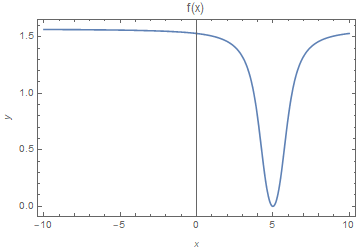
\includegraphics{images/funcao_arctang}
\caption{Gráfico gerado pela equação $f(x)=ArcTan[(x-5)^{2}]$}
\end{center}
\end{figure}

Para esse caso espera-se que o método otimizado retorne um número baixo de pontos de integração para as partes em que a função é suave e aumente conforme ocorra a oscliação.

\newpage

\begin{figure}[h]
\begin{center}
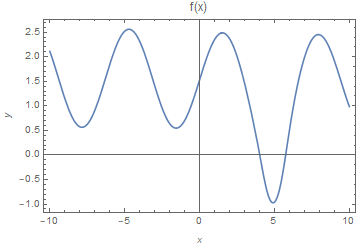
\includegraphics{images/funcao_arctangsin}
\caption{Gráfico gerado pela equação $f(x)=ArcTan[(x-5)^{2}]+Sin[x]$}
\end{center}
\end{figure}

Já pra esse caso, espera-se que o método varie os números de pontos de ingreção acompanhando a oscilação da equação, mas mantendo valores menores nas regiões entre picos e vales. 

Para os dois exemplos, foram adotados como limite de integração -10 e 10 e foi adotado um espaçamento de 0.25, ou seja, o método irá fazer o cálculo para intervalos de 0.25 dentro do limite de integração. Para os dois métodos, obtivemos os valores mostrados a seguir. Estão apresentados os valores obtidos pelo método GaussNumber, que serviu de referência para o cálculo, como também o valor obtido pelo método otimizado e por fim a difirença da integração numérica pelo método de Gauss utilizando o número resultante do método Otimizado e o valor da integral proriamente dita.

Percebe-se que os valores obtidos pelo método otimizado são, na maioria dos casos, próximos ou iguais aos valores encontrados pelo método GaussNumber, e o valor da integração utilzando esses valores são praticamente identicos com relação a integral propriamente dita.

\newpage

\newpage

\quad Na imagem da Figura 4 a seguir percebemos a diferença dos números de pontos de integração encontrados pelos dois métodos para as condições assumidas. Percebemos que os valores encontrados pelo métodos otimizado (GaussNumberII) apresenta valores próximos aos encontrados pelo método de referência (GaussNumber),

\begin{figure}[H]
\begin{center}
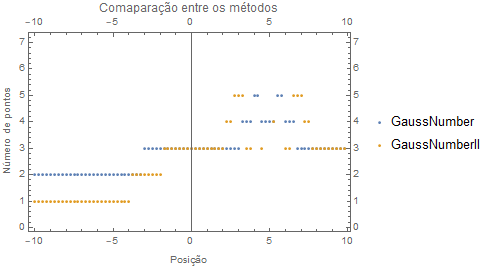
\includegraphics{images/comparacao_arctang}
\caption{Diferença entre os métodos para a função $f(x)=ArcTan[(x-5)^{2}]$.}
\end{center}
\end{figure}

\newpage
\quad Com os valores obtidos pelo método GaussNumberII foram calculadas as integrais numéricas utlizando o método da Quadratura de Gauss e os erros encontrados, quando comparado com o valor da integração numérica resolvida pelo \textit{Wolfram Mathematica}. Os resultados encontrados estão mostrados na Figura 5. Percebe-se que os valores encontrados são praticamente zero (o maior valore é da ordem de $10^{-7}$.

\begin{figure}[H]
\begin{center}
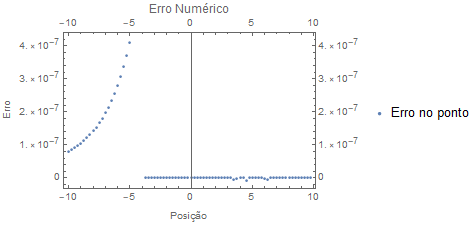
\includegraphics{images/erro_arctang}
\caption{Erro da função $f(x)=ArcTan[(x-5)^{2}]$}
\end{center}
\end{figure}

\newpage

\qquad Na imagem da Figura 6 a seguir, também é apresentada a diferença dos números de pontos de integração encontrados pelos dois métodos para as condições assumidas. Percebemos que os valores encontrados pelo métodos otimizado (GaussNumberII).Para essa situação o método otimizado também apresenta pontos próximos ao método de referência, mas para os pontos próximos as inflexções da equação o método otimizado superestima os pontos para a integração.

\begin{figure}[H]
\begin{center}
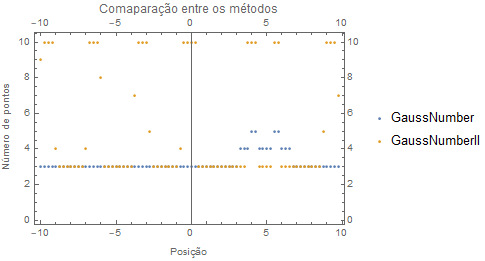
\includegraphics{images/comparacao_arctangsin}
\caption{Diferença entre os métodos para a função $f(x)=ArcTan[(x-5)^{2}]+Sin[x]$.}
\end{center}
\end{figure}

\newpage
\quad Com os valores obtidos pelo método GaussNumberII, também foram calculadas as integrais numéricas utlizando o método da Quadratura de Gauss e os erros encontrados, quando comparado com o valor da integração numérica resolvida pelo \textit{Wolfram Mathematica}. Os resultados encontrados estão mostrados na Figura 6. Percebe-se que os valores encontrados são praticamente zero (o maior valore é da ordem de $10^{-9}$.


\begin{figure}[H]
\begin{center}
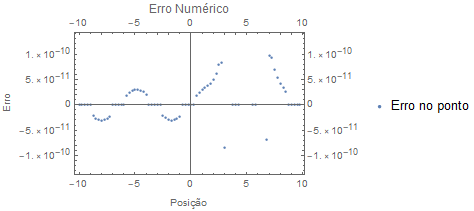
\includegraphics{images/erro_arctangsin}
\caption{Erro da função $f(x)=ArcTan[(x-5)^{2}]+Sin[x]$}
\end{center}
\end{figure}



\newpage
\section{Próximos passos}

\qquad Com os resultados apresentados percebemos que o método tem uma eficiência muito boa e quanto menor for o espaçamento da integração, melhor é o resultado do método. Contudo, ainda existem pontos que podem ser melhorados e estão sendo trabalhados. O uso da derivada numérica, por exemplo, produz uma osclição a partir da sexta derivada que invalida o seu uso, mas caso seja possível corrigir esse efeito, o método poderia utilizar mais ordens de derivada para deixar os valores de contorno ainda mais restritos e assim obter uma variação ainda melhor do método.

Ainda, a equação 3, que diz qual será o número de pontos, pode ser melhorada para algumas situações. Como foi mostrados na seção 4, para alguns intervalos o método está superestimando o número de pontos de integração, então, para essas localidades o custo computacional está sendo maior do que poderia ser.


\end{document}
